%==============================================================================
% CHAPTER 7 --- RESULTS AND EVALUATION
%==============================================================================

\chapter{Results and Evaluation}
\label{chap:results}

\chapterquote{Without data, you're just another person with an opinion.}{W. Edwards Deming}

%==============================================================================
\section{Overview}
\label{sec:results_overview}

This chapter presents the experimental evaluation of the proposed NABTA platform. The performance of each artificial intelligence component is evaluated individually, including the CNN classification model, YOLOv8 object detection model, U-Net segmentation model, Crop Recommendation model, and Smart Irrigation models. The reported results demonstrate the effectiveness of the proposed platform across all intelligent services.

All reported results are obtained using held-out test datasets that were completely separated from the training and validation datasets to ensure an unbiased evaluation of model performance.

%==============================================================================
\section{Classification Model Performance}
\label{sec:cnn_results}

\subsection{Overall Performance}
\label{subsec:cnn_acc}

The CNN classification model was evaluated on an independent test set consisting of \textbf{12,198} images covering \textbf{102} healthy and diseased plant classes collected from multiple public datasets. The model achieved an overall classification accuracy of \textbf{95.0\%}, demonstrating strong generalization across different crops, disease categories, and real-world imaging conditions.

Table~\ref{tab:cnn_metrics} summarizes the aggregate classification performance.

\begin{table}[H]
\centering
\caption{CNN Classification Model -- Overall Test Performance}
\label{tab:cnn_metrics}
\renewcommand{\arraystretch}{1.4}
\begin{tabular}{lc}
\toprule
\textbf{Metric} & \textbf{Value} \\
\midrule
Test Images & 12,198 \\
Number of Classes & 102 \\
Overall Accuracy & 95.0\% \\
Macro Precision & 95.0\% \\
Macro Recall & 94.0\% \\
Macro F1-score & 94.0\% \\
Weighted Precision & 95.0\% \\
Weighted Recall & 95.0\% \\
Weighted F1-score & 95.0\% \\
\bottomrule
\end{tabular}
\end{table}

The high weighted metrics indicate that the model performs consistently across the entire dataset, while the macro-average scores demonstrate balanced performance among the individual disease classes despite differences in class distributions.

%==============================================================================
\subsection{Representative Per-Class Performance}
\label{subsec:cnn_per_class}

Table~\ref{tab:cnn_per_class} presents representative classification results for selected plant diseases extracted from the complete classification report.

\begin{table}[H]
\centering
\caption{Representative CNN Classification Results}
\label{tab:cnn_per_class}
\renewcommand{\arraystretch}{1.4}
\begin{tabularx}{\textwidth}{X l c c c}
\toprule
\textbf{Class} &
\textbf{Plant} &
\textbf{Precision} &
\textbf{Recall} &
\textbf{F1-score} \\
\midrule

Apple Scab &
Apple &
1.00 &
1.00 &
1.00 \\

Apple Black Rot &
Apple &
1.00 &
1.00 &
1.00 \\

Apple Healthy &
Apple &
0.99 &
1.00 &
1.00 \\

Bitter Gourd Downy Mildew &
Bitter Gourd &
1.00 &
1.00 &
1.00 \\

Bitter Gourd Fusarium Wilt &
Bitter Gourd &
0.90 &
0.75 &
0.82 \\

Cassava Brown Streak Disease &
Cassava &
0.70 &
0.76 &
0.73 \\

Cassava Mosaic Disease &
Cassava &
0.93 &
0.94 &
0.94 \\

Healthy Tomato &
Tomato &
0.99 &
1.00 &
1.00 \\

\bottomrule
\end{tabularx}
\end{table}

The results demonstrate excellent recognition performance for most disease categories, with several classes achieving perfect precision and recall. Lower performance is mainly observed in visually similar diseases, particularly within cassava-related classes, where symptom similarity and class imbalance increase classification difficulty.

%==============================================================================
\subsection{Training Convergence}
\label{subsec:cnn_convergence}

Figure~\ref{fig:cnn_training} illustrates the training and validation accuracy and loss curves throughout the training process. The curves indicate stable convergence without significant overfitting, reflecting the effectiveness of the adopted preprocessing pipeline, data augmentation strategy, and regularization techniques.

\begin{figure}[H]
\centering
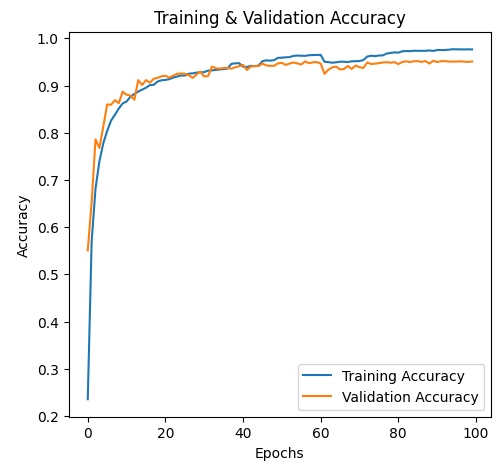
\includegraphics[width=0.48\textwidth]{assets/diagrams/cnn_accuracy_curve.png}
\hfill
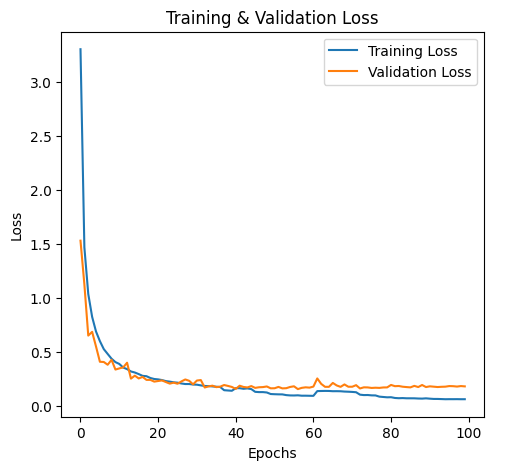
\includegraphics[width=0.48\textwidth]{assets/diagrams/cnn_loss_curve.png}
\caption{Training and Validation Accuracy and Loss Curves of the CNN Classification Model}
\label{fig:cnn_training}
\end{figure}

The training process converged smoothly, with both training and validation curves following similar trends. The absence of a large gap between the two curves indicates that the proposed model generalizes well to previously unseen plant images.
%==============================================================================
\section{YOLOv8 Detection Model Performance}
\label{sec:yolo_results}

\subsection{Overall Detection Performance}

The YOLOv8x object detection model was evaluated on the enhanced PlantDoc dataset to assess its capability in localizing diseased plant regions under real-world conditions. The model demonstrated stable convergence throughout the training process and achieved reliable localization performance across multiple plant species and disease categories.

Table~\ref{tab:yolo_metrics} summarizes the overall detection performance obtained on the validation dataset.

\begin{table}[H]
\centering
\caption{YOLOv8x Detection Performance}
\label{tab:yolo_metrics}
\renewcommand{\arraystretch}{1.4}
\begin{tabular}{lc}
\toprule
\textbf{Metric} & \textbf{Value} \\
\midrule
Model & YOLOv8x \\
Precision & 72.9\% \\
Recall & 72.6\% \\
mAP@0.50 & 78.8\% \\
mAP@0.50:0.95 & 52.8\% \\
Training Epochs & 40 \\
\bottomrule
\end{tabular}
\end{table}

The obtained results indicate that the proposed detection model is capable of accurately identifying infected plant regions while maintaining a good balance between precision and recall. The achieved mAP@0.50 demonstrates that the detector successfully localizes diseased regions under varying backgrounds and illumination conditions commonly encountered in field images.

%==============================================================================
\subsection{Training Convergence}

Throughout the training process, the training and validation losses decreased steadily, indicating stable optimization and effective learning without severe overfitting. Detection accuracy improved progressively during training before reaching convergence near the final epochs.

Figure~\ref{fig:yolo_results} illustrates the overall training performance generated by the Ultralytics framework.

\begin{figure}[H]
\centering
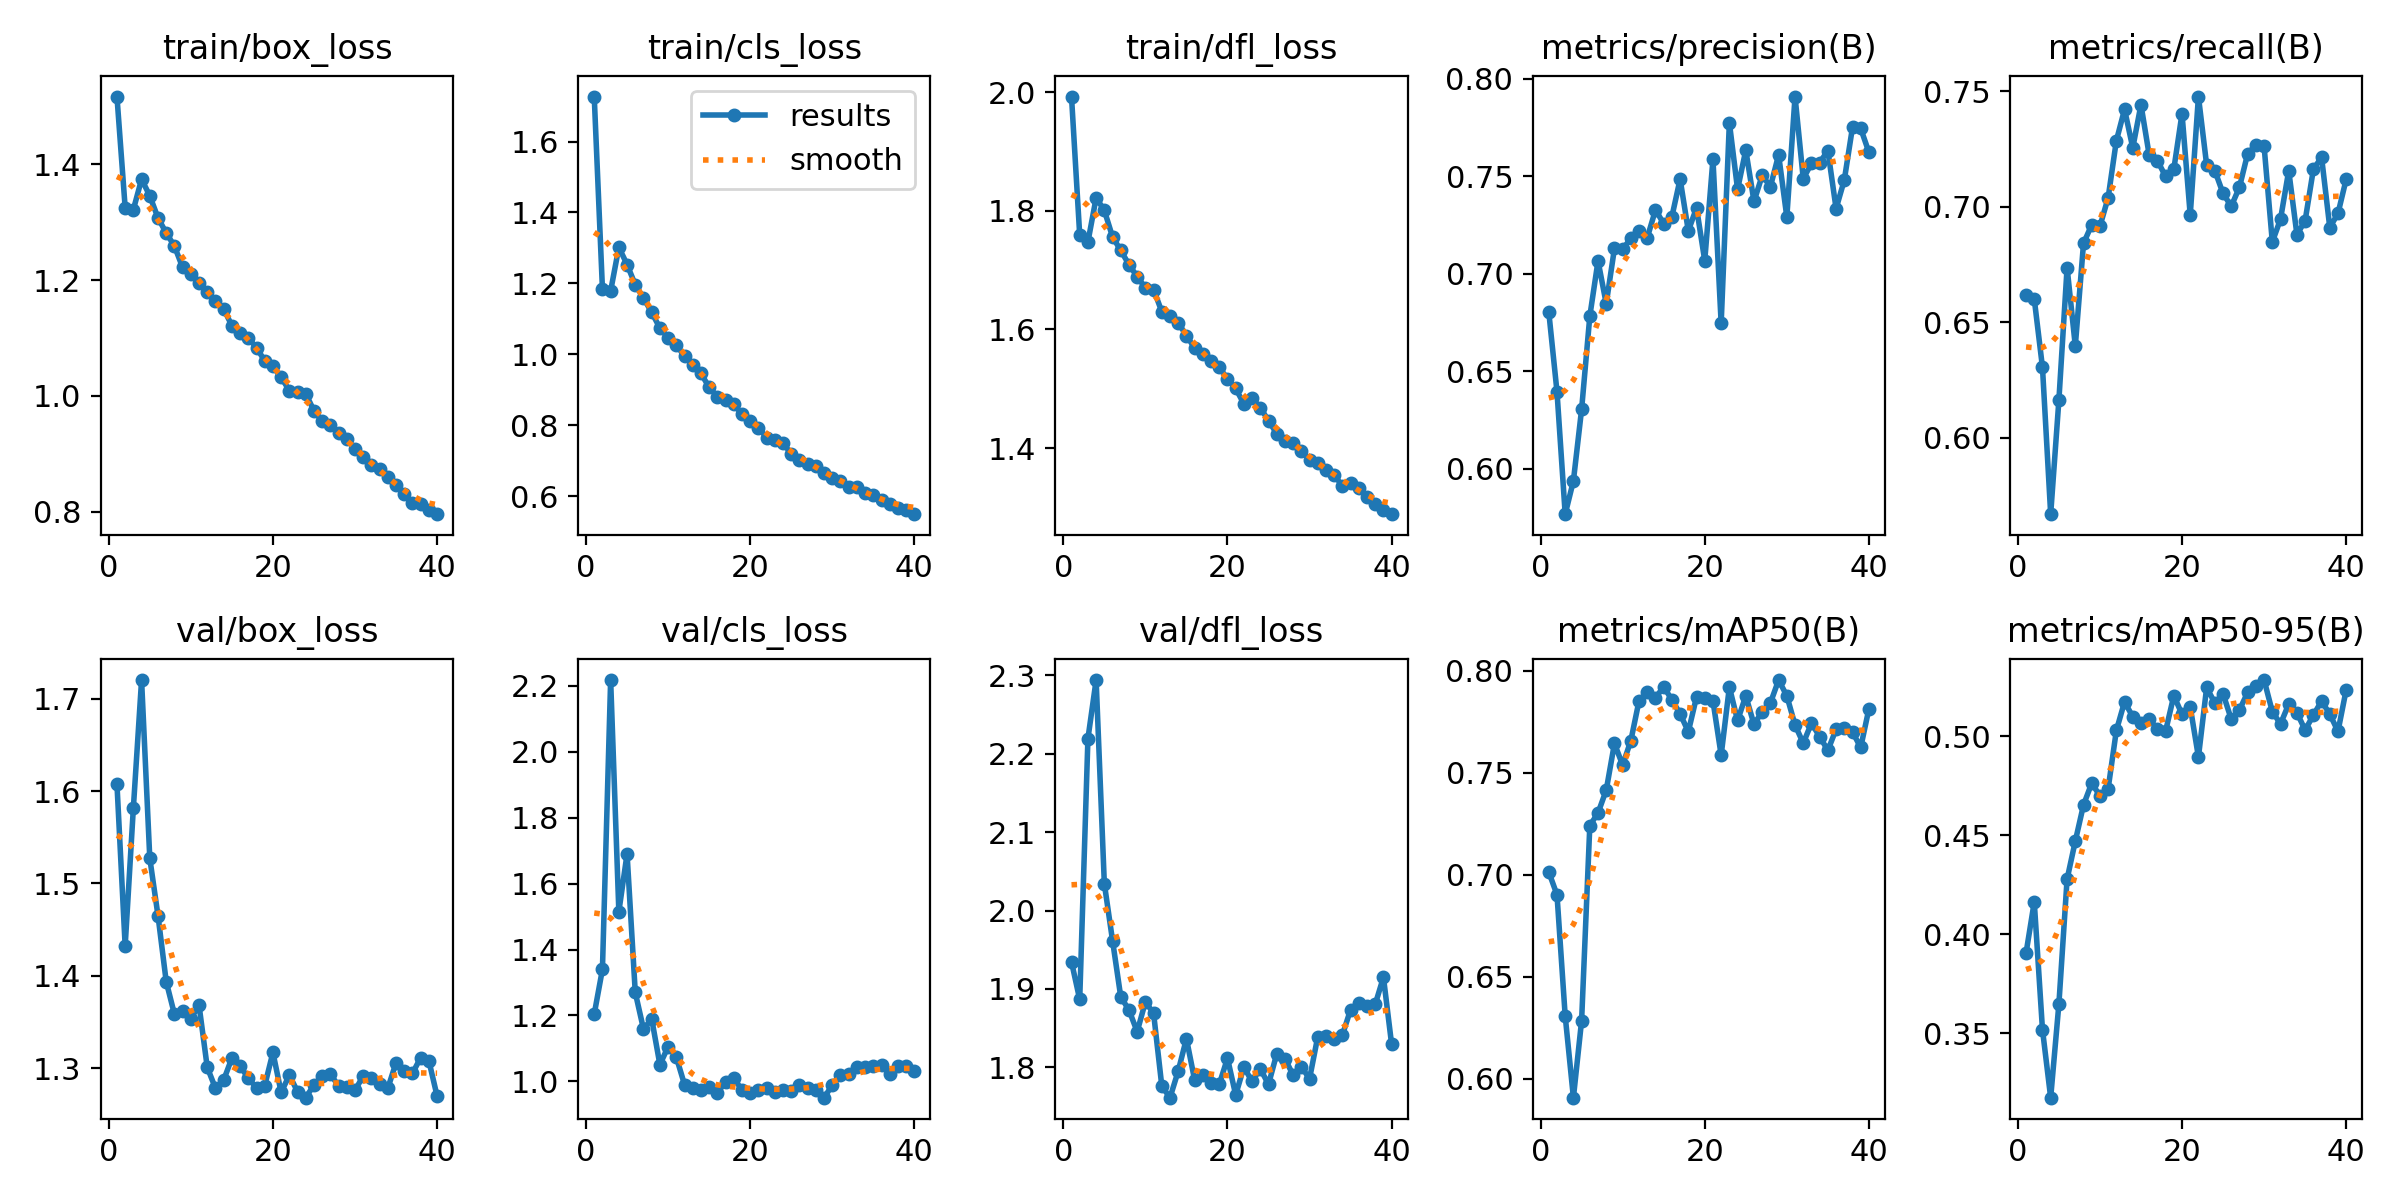
\includegraphics[width=.9\textwidth]{assets/diagrams/yolo_training_results.png}
\caption{YOLOv8x Training Results}
\label{fig:yolo_results}
\end{figure}

The precision, recall, and mAP curves consistently improved over successive epochs, confirming the effectiveness of the adopted data preprocessing, annotation refinement, and augmentation strategies.

%==============================================================================
\subsection{Detection Examples}

Figure~\ref{fig:yolo_predictions} presents representative detection examples produced by the trained YOLOv8x model.

\begin{figure}[H]
\centering
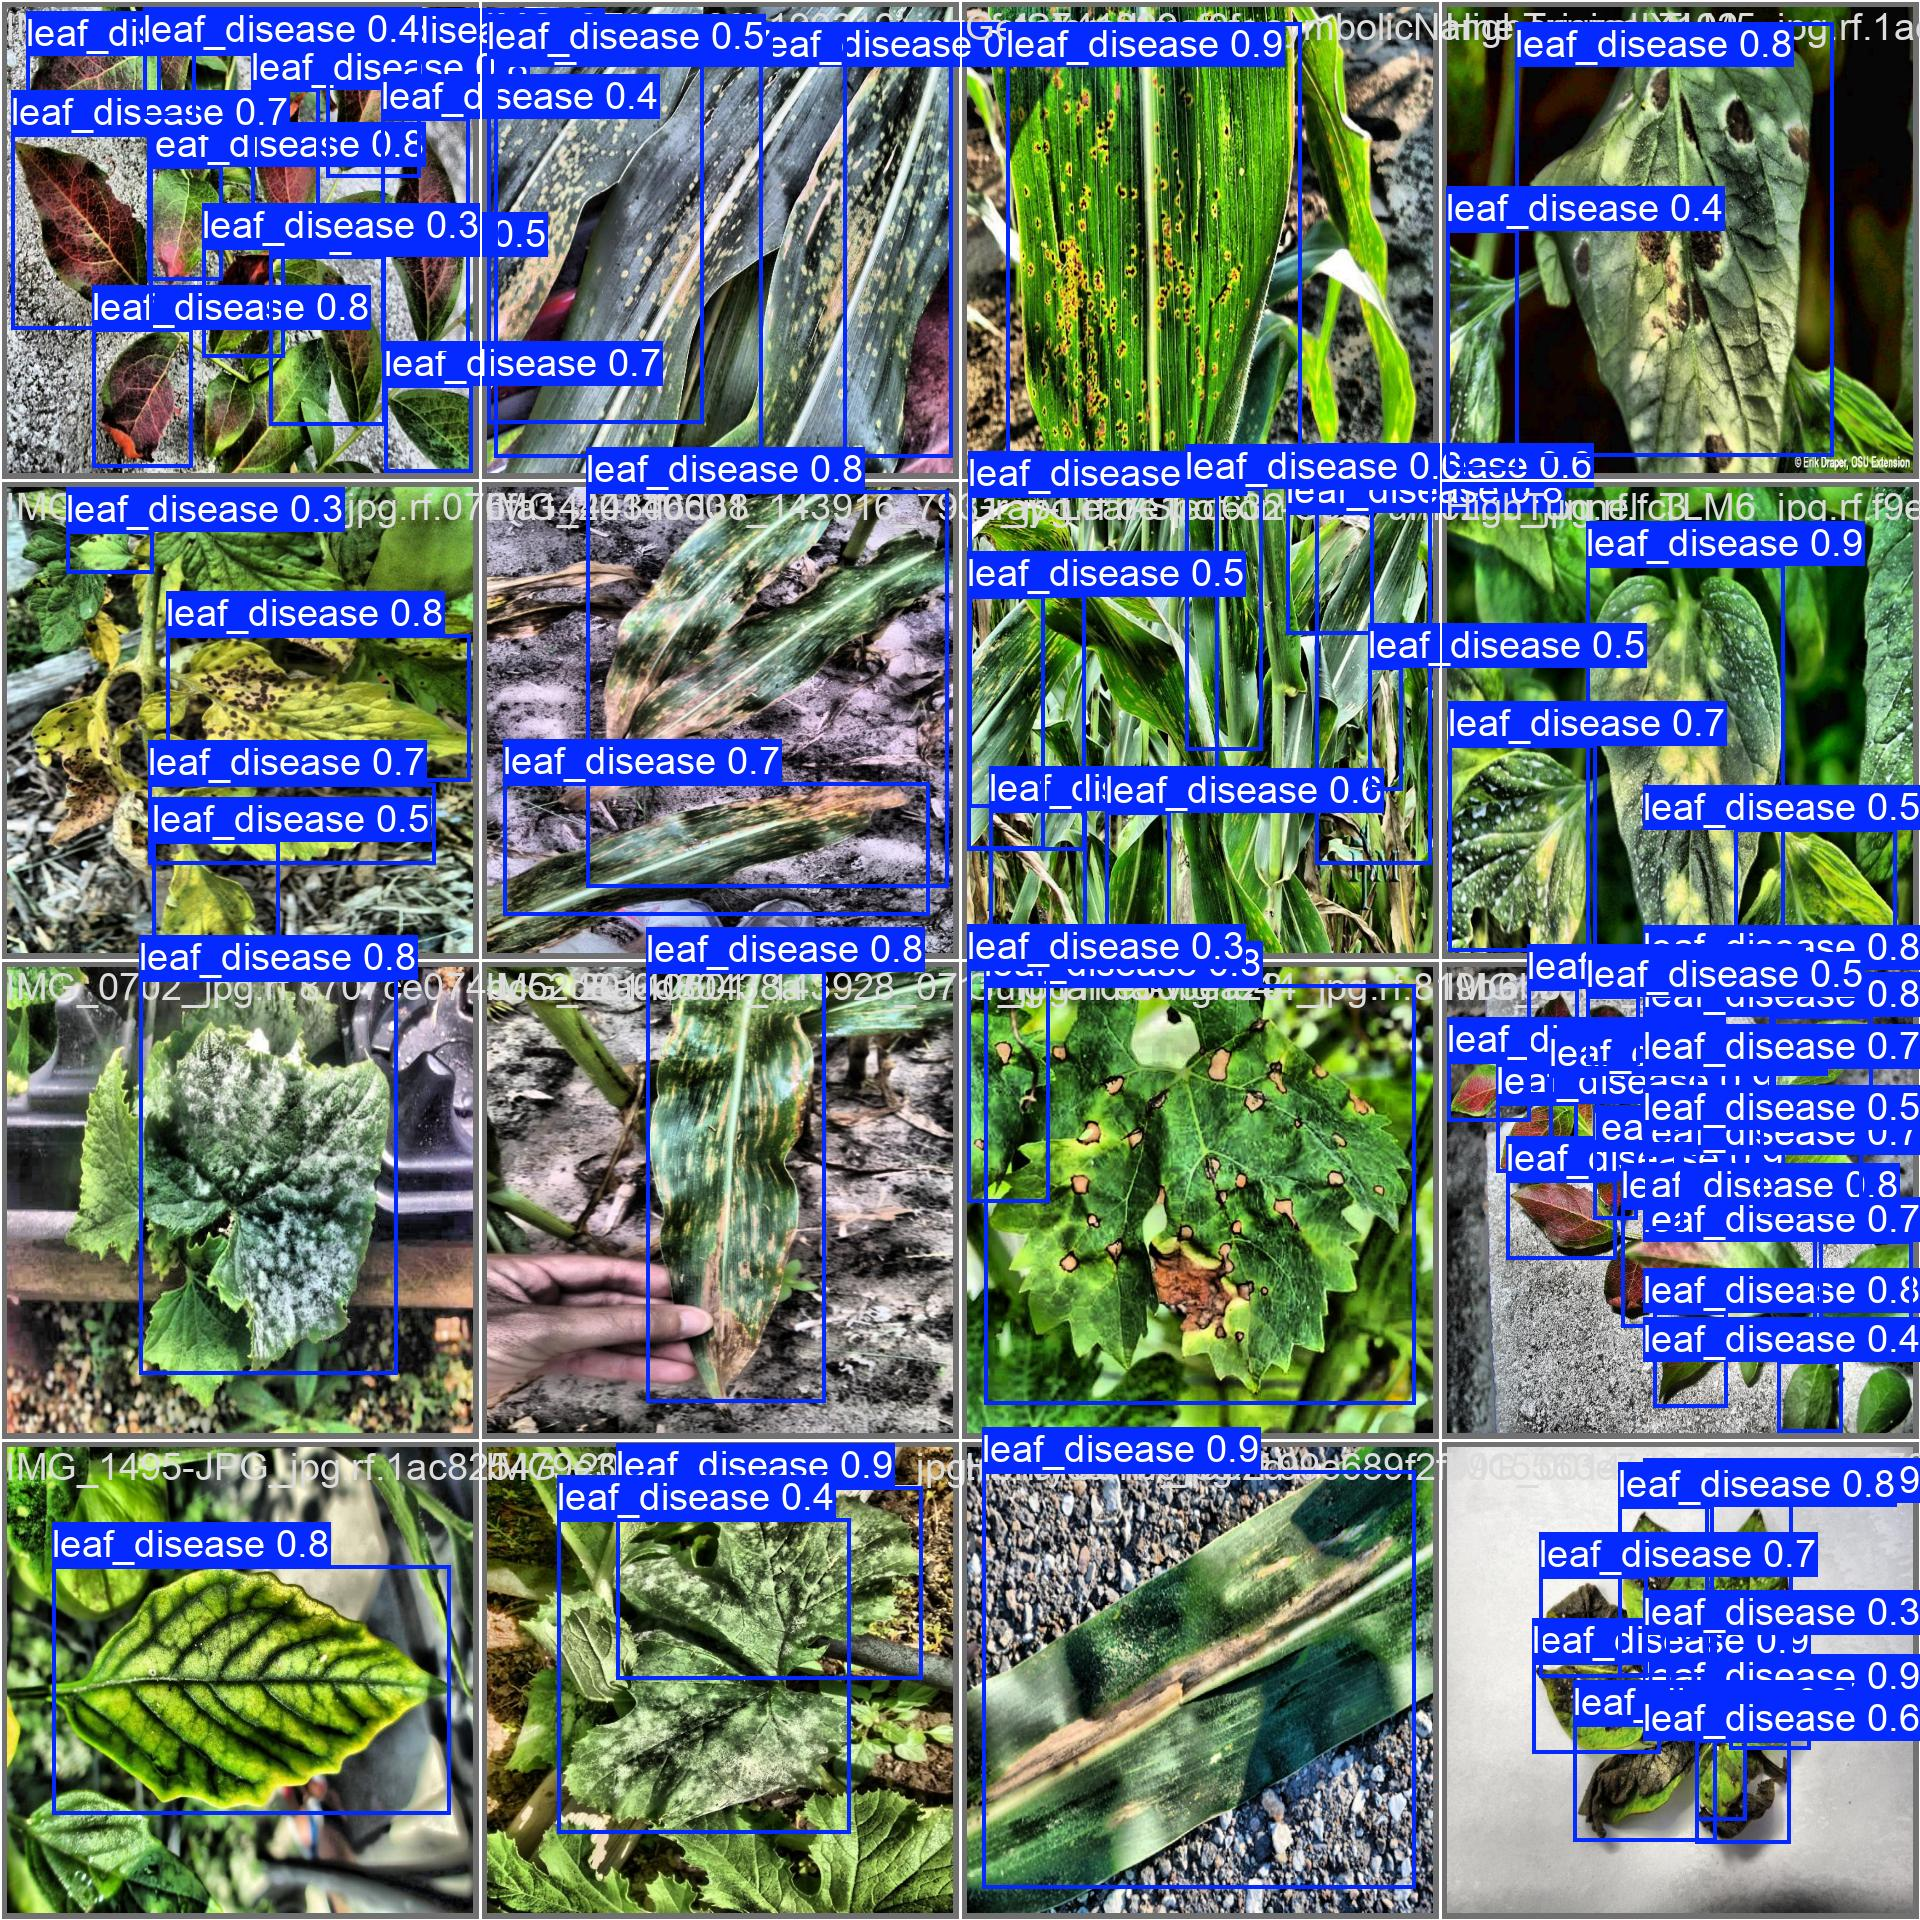
\includegraphics[width=.9\textwidth]{assets/diagrams/predictions.jpg}
\caption{Representative YOLOv8 Detection Results}
\label{fig:yolo_predictions}
\end{figure}

The model successfully localized infected leaf regions with high confidence, providing accurate regions of interest that were subsequently forwarded to the segmentation and classification stages of the NABTA pipeline.

%==============================================================================
\section{U-Net Segmentation Model Performance}
\label{sec:unet_results}

\subsection{Overall Segmentation Performance}

The proposed U-Net model with an EfficientNet-B0 encoder was evaluated using an independent validation set to measure its ability to accurately isolate plant leaves from complex backgrounds. Accurate leaf segmentation is essential because it removes irrelevant background information before disease classification, allowing the classifier to focus only on the leaf tissue.

Table~\ref{tab:unet_metrics} summarizes the overall segmentation performance achieved by the proposed model.

\begin{table}[H]
\centering
\caption{U-Net Segmentation Performance}
\label{tab:unet_metrics}
\renewcommand{\arraystretch}{1.4}
\begin{tabular}{lc}
\toprule
\textbf{Metric} & \textbf{Value} \\
\midrule
Architecture & U-Net (EfficientNet-B0 Encoder) \\
Training Epochs & 20 \\
Best Validation Accuracy & 97.89\% \\
Best Mean IoU & 94.73\% \\
Best Validation Loss & 0.1098 \\
\bottomrule
\end{tabular}
\end{table}

The segmentation model demonstrated excellent convergence throughout the training process and achieved a mean Intersection-over-Union (IoU) of \textbf{94.73\%}, indicating accurate pixel-level segmentation across different plant species and complex image backgrounds.

%==============================================================================
\subsection{Training Convergence}

Figure~\ref{fig:unet_training} illustrates the evolution of the training and validation accuracy, loss, and mean Intersection-over-Union (IoU) throughout the training process. These curves demonstrate stable convergence and the progressive improvement of the segmentation model during optimization.
\begin{figure}[H]
\centering
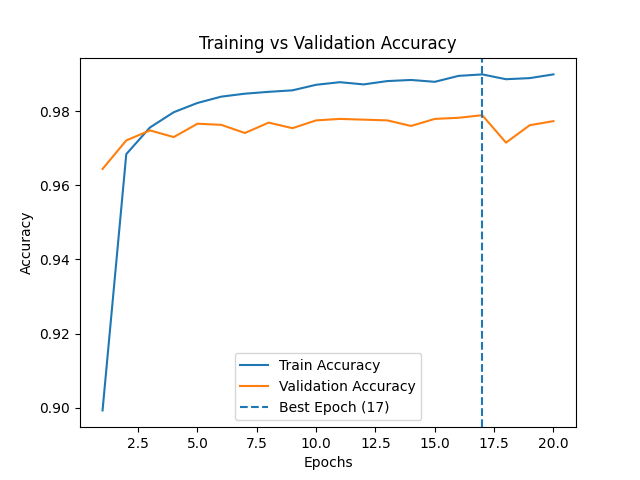
\includegraphics[width=.42\textwidth]{assets/diagrams/accuracy_curve.png}
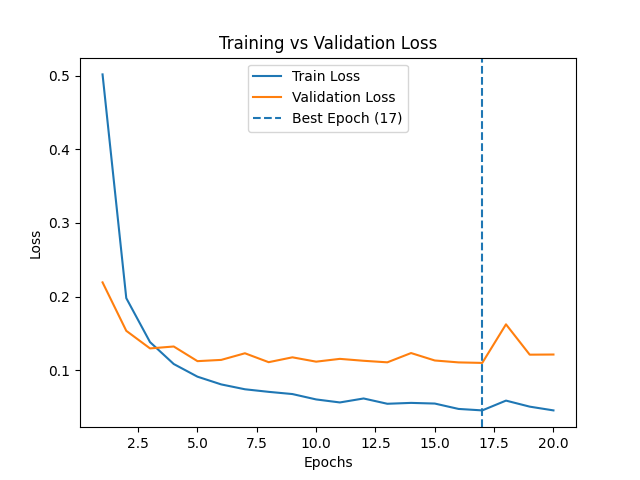
\includegraphics[width=.42\textwidth]{assets/diagrams/loss_curve.png}
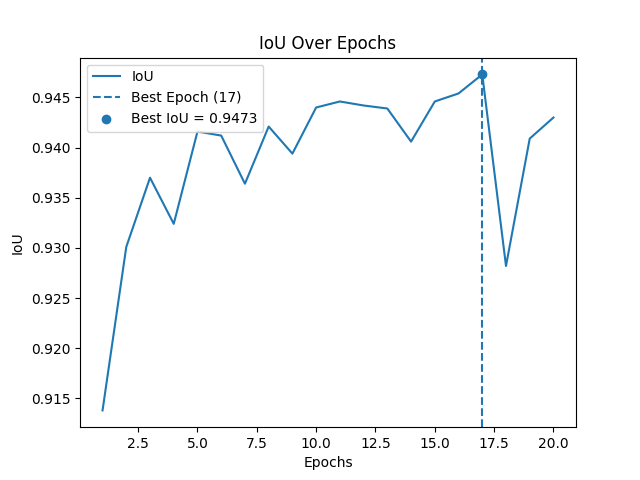
\includegraphics[width=.42\textwidth]{assets/diagrams/iou_curve.png}
\caption{Training Performance of the U-Net Segmentation Model}
\label{fig:unet_training}
\end{figure}

The training curves indicate stable optimization with no significant evidence of overfitting. Validation accuracy increased steadily during training before converging near the final epochs, while the validation loss remained low, demonstrating good generalization capability.

%==============================================================================
\subsection{Segmentation Quality}

The trained model successfully generated accurate binary masks that isolated plant leaves while suppressing background objects such as soil, shadows, surrounding vegetation, and other environmental artifacts.

Representative segmentation examples are shown in Figure~\ref{fig:unet_examples}.

\begin{figure}[H]
\centering
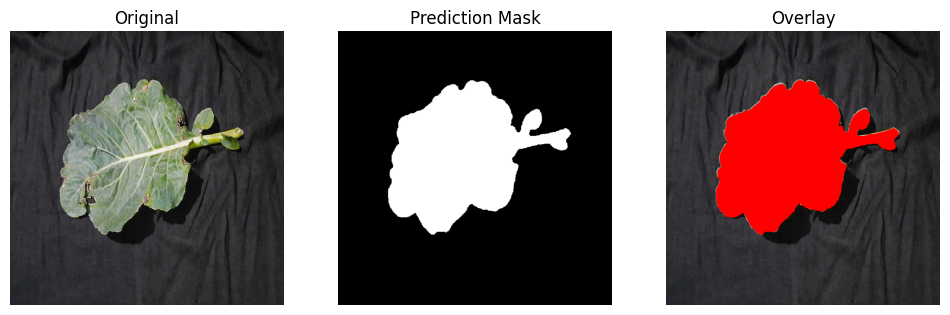
\includegraphics[width=.9\textwidth]{assets/diagrams/sample_2.png}
\caption{Representative U-Net Segmentation Results}
\label{fig:unet_examples}
\end{figure}

The generated masks preserve fine leaf boundaries and disease-affected regions, providing high-quality inputs for the downstream CNN classification model. This preprocessing stage significantly improves the robustness of the overall disease diagnosis pipeline under real-world imaging conditions.

%==============================================================================
\section{Crop Recommendation Model Performance}
\label{sec:crop_results}

\subsection{Overall Performance}

The crop recommendation model was developed using a Random Forest classifier trained on soil properties, environmental conditions, and climatic factors. The evaluation was performed using an independent test set to assess its ability to recommend the most suitable crop for different agricultural conditions.

Table~\ref{tab:crop_metrics} summarizes the overall classification performance.

\begin{table}[H]
\centering
\caption{Crop Recommendation Model Performance}
\label{tab:crop_metrics}
\renewcommand{\arraystretch}{1.4}
\begin{tabular}{lc}
\toprule
\textbf{Metric} & \textbf{Value} \\
\midrule
Model & Random Forest Classifier \\
Training Accuracy & 88.76\% \\
Test Accuracy & 85.13\% \\
Precision & 85.41\% \\
Recall & 85.13\% \\
F1-score & 85.11\% \\
Cross-validation Accuracy & 84.8\% $\pm$ 0.8\% \\
Generalization Gap & 3.6\% \\
\bottomrule
\end{tabular}
\end{table}

The relatively small generalization gap indicates that the proposed model generalizes well to unseen agricultural conditions without significant overfitting. Furthermore, the consistent cross-validation accuracy confirms the robustness and reliability of the trained classifier.

%------------------------------------------------------------------------------
\subsection{Agronomic Validation}

To improve the practical usefulness of the recommendation system, the original synthetic dataset was regenerated using agronomic crop--soil suitability rules derived from agricultural domain knowledge. Unlike the previous dataset, where soil type was assigned independently of crop type, the regenerated dataset models realistic crop-specific soil preferences.

Several representative scenarios were evaluated by keeping the nutrient and environmental conditions constant while varying only the soil type.

For rice cultivation, the prediction probability increased from \textbf{28.8\%} on sandy soil to \textbf{44.4\%} on clay soil, which is consistent with the high water-retention characteristics required for rice production. Conversely, groundnut achieved its highest prediction probability of \textbf{71.0\%} on sandy soil, while the probability decreased to \textbf{44.2\%} on clay soil under identical environmental conditions.

\begin{table}[H]
\centering
\caption{Representative Crop Recommendation Validation}
\label{tab:crop_examples}
\renewcommand{\arraystretch}{1.4}
\begin{tabular}{lcc}
\toprule
\textbf{Crop} & \textbf{Preferred Soil} & \textbf{Prediction Probability} \\
\midrule
Rice & Clay & 44.4\% \\
Rice & Sandy & 28.8\% \\
Groundnut & Sandy & 71.0\% \\
Groundnut & Clay & 44.2\% \\
\bottomrule
\end{tabular}
\end{table}

The obtained results confirm that soil characteristics now influence both the predicted probability and the ranking of recommended crops in the agronomically expected direction. Although nutrient-related features remain the dominant predictors, incorporating crop-specific soil suitability significantly improves the realism and practical usefulness of the recommendation system.

%==============================================================================
\section{Irrigation Recommendation Model Performance}
\label{sec:irrigation_results}

The irrigation module consists of two complementary machine learning models: a Random Forest classifier that determines whether irrigation is required and a Random Forest regressor that estimates crop water requirements under different environmental conditions.

%------------------------------------------------------------------------------
\subsection{Irrigation Decision Model}

Table~\ref{tab:irrigation_decision} summarizes the performance of the irrigation decision classifier.

\begin{table}[H]
\centering
\caption{Irrigation Decision Model Performance}
\label{tab:irrigation_decision}
\renewcommand{\arraystretch}{1.4}
\begin{tabular}{lc}
\toprule
\textbf{Metric} & \textbf{Value} \\
\midrule
Model & Random Forest Classifier \\
Training Accuracy & 99.37\% \\
Test Accuracy & 98.53\% \\
Precision & 98.52\% \\
Recall & 98.53\% \\
F1-score & 98.52\% \\
Generalization Gap & 0.8\% \\
\bottomrule
\end{tabular}
\end{table}

The irrigation decision classifier achieved excellent predictive performance while maintaining a very small generalization gap, indicating outstanding model stability and no observable evidence of overfitting.

%------------------------------------------------------------------------------
\subsection{Water Requirement Estimation}

The second irrigation component estimates the amount of water required by a crop using a Random Forest regression model.

\begin{table}[H]
\centering
\caption{Water Requirement Regression Performance}
\label{tab:water_requirement}
\renewcommand{\arraystretch}{1.4}
\begin{tabular}{lc}
\toprule
\textbf{Metric} & \textbf{Value} \\
\midrule
Model & Random Forest Regressor \\
Training $R^2$ & 96.81\% \\
Test $R^2$ & 95.22\% \\
Mean Absolute Error (MAE) & 13.47 mm \\
Generalization Gap & 1.59\% \\
\bottomrule
\end{tabular}
\end{table}

The Random Forest regression model achieved a test coefficient of determination ($R^2$) of \textbf{95.22\%} with a mean absolute error (MAE) of only \textbf{13.47 mm}. These results indicate that the proposed model can accurately estimate crop water requirements under different environmental conditions. The small generalization gap further confirms the robustness of the proposed regression model.

%==============================================================================
\section{Chapter Summary}

This chapter presented the experimental evaluation of all intelligent modules comprising the NABTA platform. The CNN classification model achieved an overall accuracy of \textbf{95.0\%}, while the YOLOv8x detector obtained a validation mAP@0.50 of \textbf{78.8\%}. The proposed U-Net segmentation model achieved a best mean IoU of \textbf{94.73\%}. Furthermore, the Random Forest crop recommendation model achieved a test accuracy of \textbf{85.13\%}, whereas the irrigation decision and water requirement models achieved a test accuracy of \textbf{98.53\%} and a test $R^2$ of \textbf{95.22\%}, respectively.

Overall, the obtained results demonstrate that the proposed NABTA platform provides accurate, robust, and scalable AI-powered decision support for modern smart agriculture by integrating computer vision, machine learning, explainable AI, and large language models within a unified production-ready system.
